% !TEX encoding = UTF-8 Unicode
% !TEX root = DesignDocument.tex

\section{Website}
\subsection{Considerations}

\tab The following sections will cover detailed instructions for publication and deployment of a C\# ASP.NET web application. The publication and deployment steps themselves are relatively simple but there are other factors of the project design that must be taken into consideration before publishing.  

\begin{enumerate}
    \item \textbf{Hosting Environment}

    \tab While ASP.NET Framework web applications are still only supported for production deployments on Windows IIS and Kestrel servers, ASP.NET Core 2+ web applications have been sourced to allow cross-platform production deployment. For this reason, the Visual Studio IDE provides several options for publication targets. These options include:

    \begin{itemize}
        \item Microsoft Azure Virtual Machines
        \item Microsoft Azure App Service -- This is the publication target that will be covered.
        
        \tab The Microsoft Azure related publication targets are for web applications that will run within the Azure hosted services suite. These methods of publication will directly write all new web application source code files to the associated execution directory within the Azure service.  Assuming successful publication, deployment is automatic.
        
        \item IIS, FTP
        
        \tab The IIS, FTP publication target is for directly deploying to the inetpub directory of a Windows Server that the web application developer has credentials and permissions to.  This is similar to the Azure publication target procedure except to a non-Azure Windows Server machine.
        
        \item Folder
        
        \tab The folder publication target is for writing all new web application source code to a local directory on the development machine. This allows more flexibility for custom web application publications.
    \end{itemize}
\end{enumerate}

\subsection{Publication}

\tab The following are steps for web application publication to a Microsoft Azure App Service.\\
    
    \ \\
    \tab $\bullet$ In the Visual Studio IDE, select Build $\rightarrow$ Publish.
    \begin{figure}[H] 
        \centering
        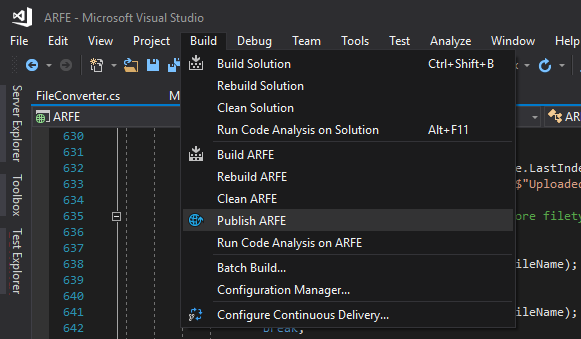
\includegraphics[scale=.6]{select_publish}
    \end{figure}
    
    \ \\
    \tab $\bullet$ If an Azure web application is already created, choose ``Select Existing''.  Otherwise, if there is no web application created, choose ``Create New''.  Choose ``Create Profile''.
    \begin{figure}[H] 
        \centering
        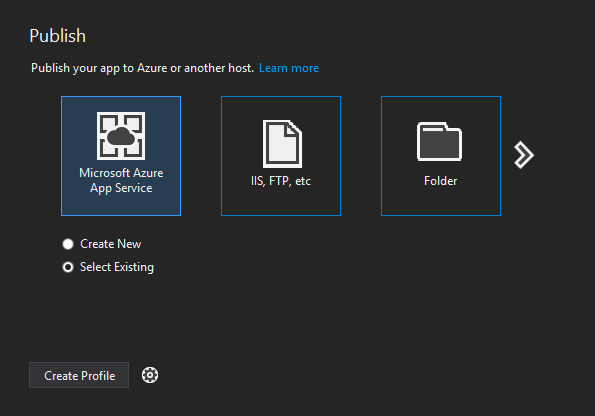
\includegraphics[scale=.6]{select_existing}
    \end{figure}
        
    \ \\
    \tab $\bullet$ This is continuing forward as if the Azure web application is already created. Select the correct web application from the menu of existing applications.
    \begin{figure}[H] 
        \centering
        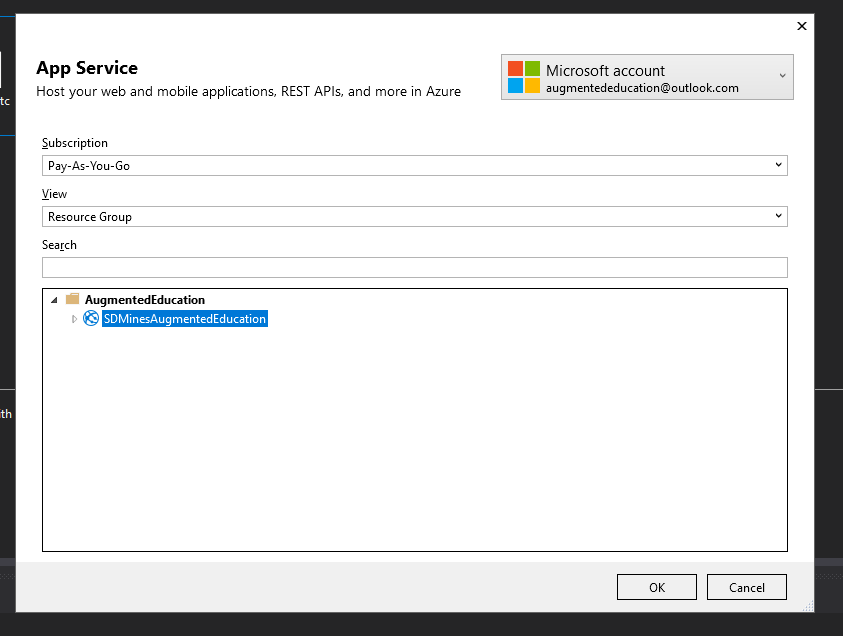
\includegraphics[scale=.6]{select_app_service}
    \end{figure}
        
    \ \\
    \tab $\bullet$ The Summary settings of the selected web application publishing profile should now be shown.
    \begin{figure}[H] 
        \centering
        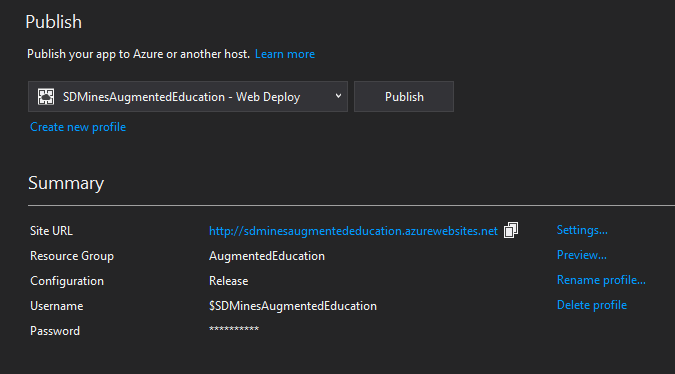
\includegraphics[scale=.6]{review_settings}
    \end{figure}
    
    \ \\
    \tab $\bullet$ Click ``Settings...'' to review the publication profile settings and ensure the fields are filled out similarly as to what is shown.
    \begin{figure}[H] 
        \centering
        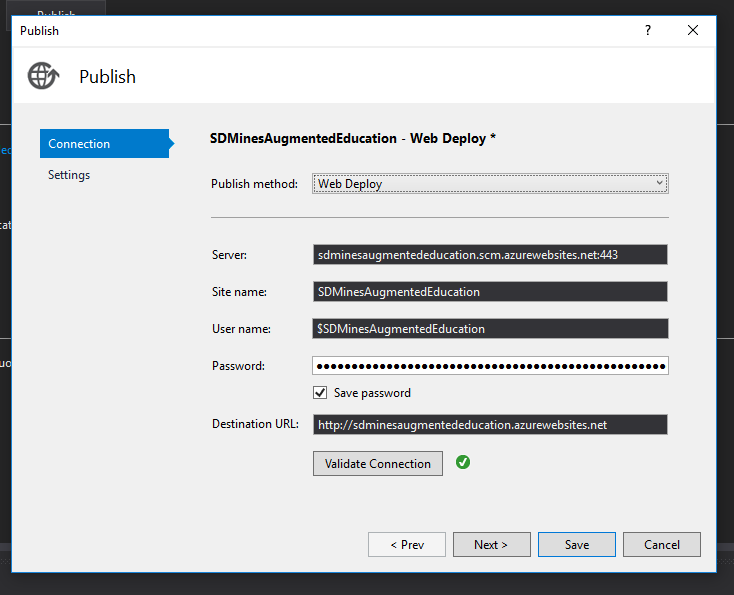
\includegraphics[scale=.6]{connection}
    \end{figure}
    
    \ \\
    \tab $\bullet$ Click ``Next'' to review the configuration settings and ensure the fields are filled out similarly as to what is shown.
    \begin{figure}[H] 
        \centering
        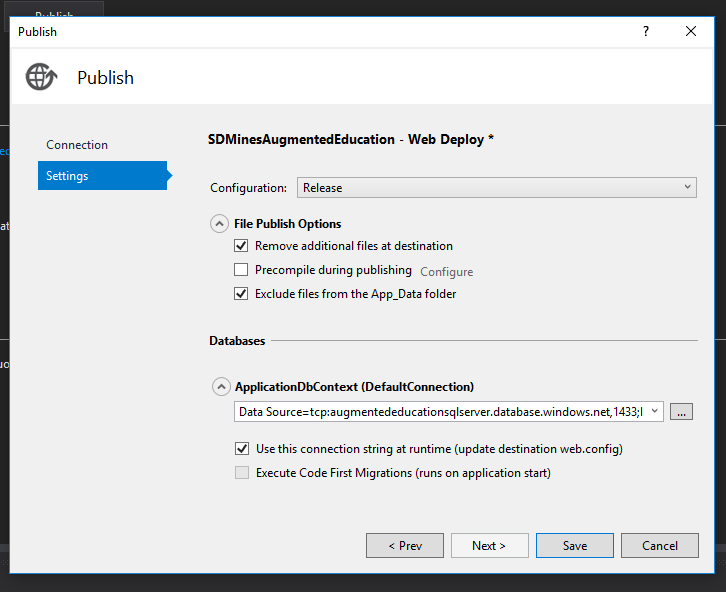
\includegraphics[scale=.6]{settings}
    \end{figure}
    
    \ \\
    \tab $\bullet$ Click ``Save'' on the configuration window and then ``Publish'' on the main Publish screen.
    \begin{figure}[H] 
        \centering
        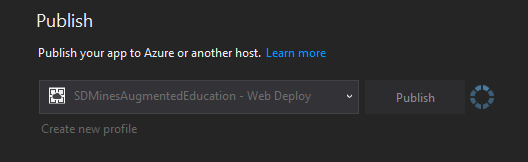
\includegraphics[scale=.6]{publish}
    \end{figure}
    
    \ \\
    \tab $\bullet$ The status of the publication will be displayed in the ``Web Publish Activity'' window.  Any publication errors will be reported here during the publication process.
    \begin{figure}[H] 
        \centering
        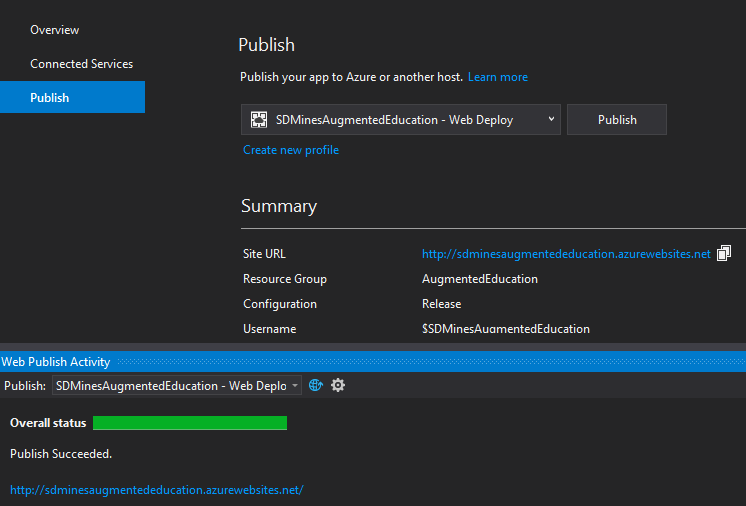
\includegraphics[scale=.6]{publish_succeeded}
    \end{figure}
    \ \\
\subsection{Deployment}